% fig_ar_tdead.tex
% TR-36: Arc deionisation time and dead time vs k_ibr
%
% X-axis: k_ibr [0.05, 1.05]
% Y-axis: time [ms]
%
% Curves:
%   T_arc  = 400 * sqrt(I_fault/10kA) * 1000  ms   (blue)
%   T_dead = T_arc + 50 ms                          (teal, dashed)
%
% Horizontal lines:
%   T_mem  = 100 ms  (red dashed) — memory expires
%   T_dead_max = 575 ms  (orange dashed) — IBR ride-through limit
%
% Shaded:
%   T_dead < T_dead_max: feasible AR window (green)
%   T_dead > T_dead_max: infeasible (red)

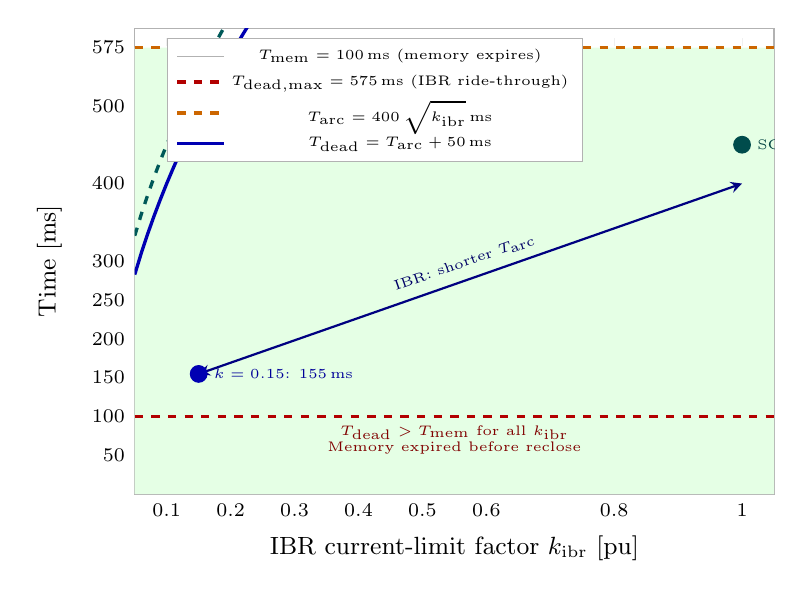
\begin{tikzpicture}
\begin{axis}[
  name        = tdax,
  width       = 0.80\textwidth,
  height      = 7.5cm,
  xlabel      = {IBR current-limit factor $k_\mathrm{ibr}$ [pu]},
  ylabel      = {Time [ms]},
  xlabel style= {font=\small},
  ylabel style= {font=\small, yshift=4pt},
  xmin=0.05, xmax=1.05,
  ymin=0, ymax=600,
  xtick       = {0.10,0.20,0.30,0.40,0.50,0.60,0.80,1.00},
  ytick       = {50,100,150,200,250,300,400,500,575},
  xticklabel style={font=\scriptsize},
  yticklabel style={font=\scriptsize},
  grid        = major,
  grid style  = {gray!12, dashed},
  tick style  = {draw=none},
  axis line style={gray!60},
  legend style={at={(0.05,0.98)}, anchor=north west, font=\tiny,
                draw=gray!60, fill=white},
]

%% ── Feasible region (T_dead <= 575 ms) ───────────────────────────────────────
\addplot[fill=green!10, draw=none]
  coordinates {(0.05,0) (1.05,0) (1.05,575) (0.05,575)} \closedcycle;

%% ── T_mem line ────────────────────────────────────────────────────────────────
\addplot[red!70!black, very thick, dashed, mark=none]
  coordinates {(0.05,100) (1.05,100)};
\addlegendentry{$T_\mathrm{mem}=100$\,ms (memory expires)}

%% ── T_dead_max line ──────────────────────────────────────────────────────────
\addplot[orange!80!black, very thick, dashed, mark=none]
  coordinates {(0.05,575) (1.05,575)};
\addlegendentry{$T_\mathrm{dead,max}=575$\,ms (IBR ride-through)}

%% ── T_arc curve ──────────────────────────────────────────────────────────────
\addplot[blue!70!black, very thick, mark=none,
         domain=0.05:1.05, samples=101]
  ({x}, {400*sqrt(x*10)*1});
\addlegendentry{$T_\mathrm{arc}=400\,\sqrt{k_\mathrm{ibr}}\,\mathrm{ms}$}

%% ── T_dead curve ─────────────────────────────────────────────────────────────
\addplot[teal!70!black, very thick, dashed, mark=none,
         domain=0.05:1.05, samples=101]
  ({x}, {400*sqrt(x*10) + 50});
\addlegendentry{$T_\mathrm{dead}=T_\mathrm{arc}+50$\,ms}

%% ── Key point annotations ────────────────────────────────────────────────────
% At k=0.15: T_dead = 205 ms
\addplot[mark=*, mark size=3pt, blue!70!black]
  coordinates {(0.15, 154.9)};
\node[blue!60!black, font=\tiny, right=2pt]
  at (axis cs:0.15, 154.9) {$k=0.15$: 155\,ms};

% At k=1.00: T_dead = 450 ms
\addplot[mark=*, mark size=3pt, teal!60!black]
  coordinates {(1.00, 450)};
\node[teal!50!black, font=\tiny, right=2pt]
  at (axis cs:1.00, 450) {SG: 450\,ms};

%% ── "T_dead always > T_mem" zone label ───────────────────────────────────────
\node[red!50!black, font=\tiny, align=center]
  at (axis cs:0.55, 70)
  {$T_\mathrm{dead}>T_\mathrm{mem}$ for all $k_\mathrm{ibr}$\\Memory expired before reclose};

%% ── IBR advantage annotation ─────────────────────────────────────────────────
\draw[<->, >=stealth, blue!50!black, thick]
  (axis cs:0.15, 154.9) -- (axis cs:1.00, 400)
  node[midway, above, sloped, font=\tiny, blue!40!black]
  {IBR: shorter $T_\mathrm{arc}$};

\end{axis}
\end{tikzpicture}
